\chapter{Socioeconomic Environment}\label{chap:8}
\section{Social Impact}\label{sec:chap6_soc}

The social impact of this project is something that must be analyzed as this type of technology even though have been around for some time, at the pace it is evolving can soon cause them to truly seem human like. This is a problem or at least something that must be taken account as people don’t like to feel fooled, if we consider the impact Google Duplex has had since it launched, people where amazed and scared of the fact that the assistant used human behavior while talking like humming while it searched for information.\\

Other things to consider as a social impact would be the other way around, the vulnerability of chatbots, as it is a machine interacts with people it must be correctly designed to stop users from accessing privileged information or extracting information from the system. Another factor is the fact that some chatbots learn from interactions, if not careful these interactions may be racist or contain offensive content that may cause the chatbot to become a part of that it learns.\\

The positive impact of this project socially is the fact that when fully developed will provide a way for connecting with new people and make it easier for people to train without having to spend a large amount of money or time to learn how to do exercises correctly or what routes are better to run.\\

Another social impact of this project if it catches the user’s attention and use it regularly is that the health benefits of training will compensate indirectly with health issues caused by obesity or heart problems.


\section{Economic Impact}\label{sec:chap6_eco}

There are two sides to the economic impact this project may have in society, first of all would be the increase in users using this platform will highly likely increase the amount of users going to gyms, with this the profits for these gyms will also increase, creating not only more jobs to support the influx of users but maybe more opportunities for gym openings. Also, by providing a cheaper tool for users, the cost of hiring a personal trainer is reduced to the fee for using the service this project would provide.\\

The other side of the economic impact would be how this project affects personal trainers, as can be verified in the query done in section 4.1.1[REFERENCE] 53,1\% prefer the services of a professional rather than a chatbot, this means that there is still a market for personal trainers, still we think that the development of this project could impact negatively on the people working as personal trainers, but comparing the pros and cons we consider that the benefits in the economy compensates any negative impact on the sector.


\begin{center}
	\begin{figure}[h!]
		\centering
		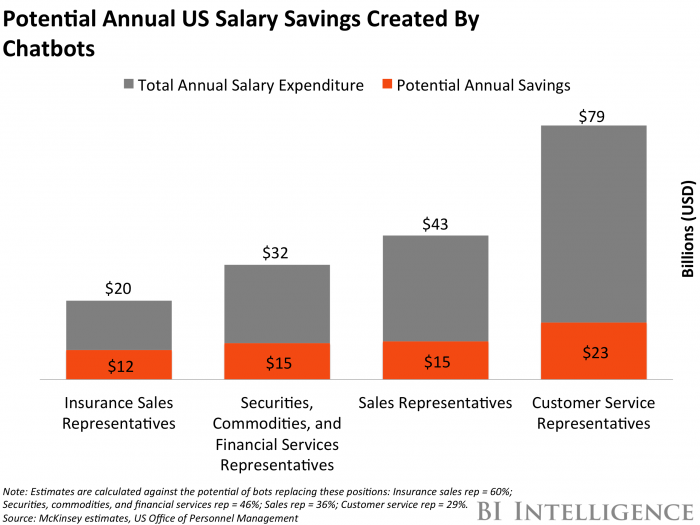
\includegraphics[scale=0.7]{./images/6-chat-sav}
		\caption{Savings Caused by Chatbots}
		\label{6_chat_sav}
	\end{figure}
\end{center}

As can be seen in the figure, based on US salaries the savings caused by chatbots can account for billions in expenses, those billions saved can be used to further invest on a company’s growth and by that impacting positively on the global economy.